\scanpage{137}

\uline{Corollary} Suppose that the homomorphism $M\handwritten{\longrightarrow}M\otimes_{k}M$ induces a homomorphism $M\otimes_{(A,\handwritten{\Delta}_{A})}(A\otimes_{k}A)\quad M\otimes_{k}M\deleted{\unsure{,|x}}$ \deleted{thus by reduction} which is an \uline{isomorphism} Then the homomorphism $u\handwritten{\unsure{\mathrel{\vert\! -\!\vert}|\mapsto}}u.e$ from $A$ to $M$ is an isomorphism for all the structures.

It suffices to prove that the rank $\inserted{n}$ of $M$ over $A$ is $1$. Now this rank of $M\otimes_{k}M$ over $A\otimes_{k}A$ is $n^{2}$, and we shall have $n=n^{2}$, i.e. $n(n-1)=0$ whence, since $n\handwritten{\not}=0$, $n=1$. This only works if one knows that the rank is \unsure{\rlap{m}finite|finite|mini}. But one can also say that the diagonal map for $\overset{\handwritten{-}}{M}$, deduced from that of $M$ by passage to the quotient (NB $\overset{\handwritten{-}}{M}\otimes\overset{\handwritten{-}}{M}=(M\rlap{\(M\)}\otimes_{k}M)\otimes_{(A\otimes_{k}A)}k$) is \uline{surjective}, hence bijective since it is unital, hence every element of $\overset{\handwritten{-}}{M}\otimes\overset{\handwritten{-}}{M}$ is of the form $\overset{\handwritten{-}}{e}\otimes x$, which is only possible if $\overset{\handwritten{-}}{e}$ generates $\overset{\handwritten{-}}{M}$.

This shows that the conjecture of local triviality r\unsure{\rlap{u}a|a}\rlap{n}ised in my notes on $\otimes$-categories works if the bialgebra $A$ en\rlap{f}visaged is finite over $k$,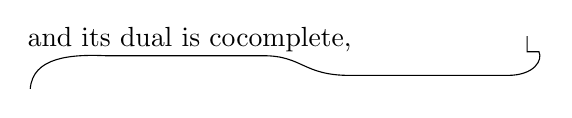
\begin{tikzpicture}[baseline=-.5ex,x=1cm,y=1cm]
\node[anchor=west,inner sep=0] at (0,.4) {\inserted{and its dual is cocomplete,}};
\draw (.04,-.22) .. controls (.07,.18) and (.55,.22) .. (1,.2) -- (3,.2) .. controls (3.5,.2) and (3.5,-.05) .. (4.1,-.05) -- (6.1,-.05) .. controls (6.45,-.05) and (6.55,.15) .. (6.5,.25) -- (6.35,.25) -- (6.35,.45);
\end{tikzpicture} \uline{provided that} the\deleted{a} algebra $B$ admits an algebra homomorphism to $k$ (or an extension of $k$), i.e. provided that $B$ is not identical to its commutator ideal.
% archive sheet number: 136
